\documentclass[12pt, a4paper]{ctexart}

%========================================
% 宏包引入
%========================================
\usepackage[margin=2.5cm]{geometry}
\usepackage{amsmath, amssymb, amsthm, mathtools}
\usepackage{xcolor}
\usepackage{graphicx}
\usepackage{tikz}
\usepackage{pgfplots}
\usepackage{tcolorbox}
\usepackage{booktabs}
\usepackage{hyperref}
\usepackage{fancyhdr}
\usepackage{algorithm}
\usepackage{algorithmic}
\usepackage{bm}
\usepackage{listings}

% 设置绘图库
\usetikzlibrary{arrows.meta, positioning, calc, shapes, decorations.pathreplacing, patterns, automata, 3d}
\pgfplotsset{compat=1.18}

%========================================
% 代码高亮设置
%========================================
\lstset{
    language=Python,
    basicstyle=\ttfamily\small,
    keywordstyle=\color{blue}\bfseries,
    commentstyle=\color{gray},
    stringstyle=\color{red},
    numbers=left,
    numberstyle=\tiny\color{gray},
    breaklines=true,
    frame=single,
    backgroundcolor=\color{gray!5}
}

%========================================
% 自定义颜色与环境
%========================================
\definecolor{myblue}{RGB}{0, 102, 204}
\definecolor{myred}{RGB}{204, 0, 0}
\definecolor{mygreen}{RGB}{0, 153, 76}
\definecolor{mypurple}{RGB}{128, 0, 128}
\definecolor{myorange}{RGB}{255, 140, 0}
\definecolor{gpugreen}{RGB}{118, 185, 0}

% 板书环境
\tcbuselibrary{skins, breakable}
\newtcolorbox{blackboard}[1][]{
    colback=gray!10,
    colframe=black!70,
    fonttitle=\bfseries,
    title={#1},
    boxrule=0.5mm,
    sharp corners,
    breakable
}

% 直觉与洞察
\newtcolorbox{insight}[1][]{
    colback=yellow!10,
    colframe=orange!60!black,
    fonttitle=\bfseries,
    title={直觉：#1},
    breakable
}

% 关键结论
\newtcolorbox{keypoint}[1][]{
    colback=myblue!5,
    colframe=myblue,
    fonttitle=\bfseries,
    title={核心结论：#1},
    breakable
}

% GPU要点
\newtcolorbox{gpubox}[1][]{
    colback=gpugreen!10,
    colframe=gpugreen!70!black,
    fonttitle=\bfseries,
    title={GPU视角：#1},
    breakable
}

% 复杂度分析
\newtcolorbox{complexitybox}[1][]{
    colback=myred!5,
    colframe=myred!70!black,
    fonttitle=\bfseries,
    title={复杂度：#1},
    breakable
}

% 实验环境
\newtcolorbox{experiment}[1][]{
    colback=mypurple!5,
    colframe=mypurple,
    fonttitle=\bfseries,
    title={实验：#1},
    breakable
}

% 定义与定理
\newtheorem{theorem}{定理}[section]
\newtheorem{lemma}[theorem]{引理}
\newtheorem{definition}[theorem]{定义}
\newtheorem{proposition}[theorem]{命题}
\newtheorem{corollary}[theorem]{推论}
\newtheorem{example}[theorem]{例}

%========================================
% 页眉页脚
%========================================
\pagestyle{fancy}
\fancyhf{}
\fancyhead[L]{优化算法：从理论到大规模实践}
\fancyhead[R]{第2周：凸优化与KKT}
\fancyfoot[C]{\thepage}

%========================================
% 文档开始
%========================================
\begin{document}

\begin{center}
{\LARGE\bfseries 第2周：凸优化与KKT条件}

\vspace{0.5cm}
{\large 从NP-Hard到多项式时间：凸性的魔力}
\end{center}

\tableofcontents
\newpage

%========================================
\section*{本讲导读}
%========================================

\begin{blackboard}[内容层次]

\textbf{核心内容}（课堂必讲，约 90 分钟）：
\begin{itemize}
    \item 凸集、凸函数的定义与判定（一阶/二阶条件）
    \item 凸优化的标准形式，LP/QP 例子
    \item Lagrangian、对偶函数、弱对偶
    \item KKT 条件（四个条件 + 直觉）
    \item 实验 2a/2b
\end{itemize}

\textbf{重要证明}（标注 $\bigstar$，选讲或自学）：
\begin{itemize}
    \item 一阶条件、二阶条件的证明
    \item KKT 条件的推导
    \item Logistic 回归的凸性证明
\end{itemize}

\textbf{进阶内容}（标注 $\bigstar$，适合优秀学生）：
\begin{itemize}
    \item MDP 与线性规划：序贯决策问题的优化视角
    \item Bellman 方程 $\to$ LP 不等式
    \item LP 对偶 $\leftrightarrow$ 值函数 vs 占用度量
\end{itemize}

\textbf{扩展内容}（自学材料）：
\begin{itemize}
    \item SOCP、SDP 的详细例子
    \item 机器学习视角的深入讨论
    \item 影子价格的完整推导
\end{itemize}

\end{blackboard}

\begin{blackboard}[数学记号]

\begin{center}
\begin{tabular}{c|l}
记号 & 含义 \\
\hline
$\nabla f(x)$ & 梯度（列向量） \\
$\nabla^2 f(x)$ & Hessian 矩阵 \\
$A \succeq 0$ & $A$ 半正定（所有特征值 $\geq 0$） \\
$A \succ 0$ & $A$ 正定（所有特征值 $> 0$） \\
$\langle A, B \rangle$ & 矩阵内积 $= \text{tr}(A^T B)$ \\
$p^*$ & 原问题最优值 \\
$d^*$ & 对偶问题最优值 \\
$\lambda, \nu$ & Lagrange 乘子
\end{tabular}
\end{center}

\end{blackboard}

%========================================
\section{回顾：从复杂度到结构}
%========================================

\begin{blackboard}[第1周的核心结论]

\textbf{问题的难度层级}：

\begin{center}
\begin{tikzpicture}[scale=0.9]
    \draw[->, thick] (0, 0) -- (12, 0);
    \node[below] at (12, 0) {难度};
    
    \fill[green!30] (0, 0.3) rectangle (4, 0.8);
    \node at (2, 0.55) {\small P（高效）};
    
    \fill[yellow!30] (4, 0.3) rectangle (7, 0.8);
    \node at (5.5, 0.55) {\small NP};
    
    \fill[orange!30] (7, 0.3) rectangle (9, 0.8);
    \node at (8, 0.55) {\small NP-Hard};
    
    \fill[red!30] (9, 0.3) rectangle (12, 0.8);
    \node at (10.5, 0.55) {\small 不可判定};
    
    % 标注
    \node[below, font=\small] at (2, -0.3) {排序、最短路};
    \node[below, font=\small] at (5.5, -0.3) {SAT、TSP};
    \node[below, font=\small] at (8, -0.3) {一般优化};
    \node[below, font=\small] at (10.5, -0.3) {停机问题};
\end{tikzpicture}
\end{center}

\textbf{关键问题}：一般优化是 NP-Hard，我们怎么办？

\end{blackboard}

\begin{blackboard}[从NP-Hard逃脱的方法]

\textbf{方法1}：接受近似解（启发式算法）

\textbf{方法2}：利用问题的\textbf{特殊结构}

\begin{center}
\begin{tabular}{c|c|c}
结构 & 复杂度 & 例子 \\
\hline
无结构（一般） & NP-Hard & 一般非线性优化 \\
\textbf{凸} & \textbf{P} & \textbf{凸优化（本周重点）} \\
线性 & P & 线性规划 \\
图结构 & 取决于具体问题 & 最短路、最小生成树
\end{tabular}
\end{center}

\textbf{本周主题}：\textbf{凸性}是最重要的``好结构''

\end{blackboard}

\begin{insight}[凸性为什么重要？]

\textbf{优化的终极梦想}：给我一个函数，我想找它的最小值

\textbf{噩梦}：函数有很多局部最小值，你找到的可能不是全局最优

\begin{center}
\begin{tikzpicture}[scale=0.8]
    % 非凸函数
    \begin{scope}
        \draw[->] (0, 0) -- (5, 0) node[right] {$x$};
        \draw[->] (0, 0) -- (0, 3) node[above] {$f(x)$};
        \draw[thick, blue, domain=0.3:4.7, samples=100] plot (\x, {0.5*(\x-1)*(\x-2.5)*(\x-4) + 2});
        \fill[red] (1, 2) circle (2pt);
        \fill[red] (4, 2) circle (2pt);
        \fill[green!50!black] (2.5, 0.8) circle (2pt);
        \node[below] at (2.5, -0.3) {非凸：多个极值点};
    \end{scope}
    
    % 凸函数
    \begin{scope}[xshift=7cm]
        \draw[->] (0, 0) -- (5, 0) node[right] {$x$};
        \draw[->] (0, 0) -- (0, 3) node[above] {$f(x)$};
        \draw[thick, blue, domain=0.3:4.7, samples=100] plot (\x, {0.3*(\x-2.5)*(\x-2.5) + 0.5});
        \fill[green!50!black] (2.5, 0.5) circle (2pt);
        \node[below] at (2.5, -0.3) {凸：唯一极值点};
    \end{scope}
\end{tikzpicture}
\end{center}

\textbf{凸的礼物}：局部最优 = 全局最优！

\end{insight}

%========================================
\section{凸集与凸函数}
%========================================

\subsection{凸集的定义}

\begin{blackboard}[凸集：几何定义]

\begin{definition}[凸集]
集合 $C \subseteq \mathbb{R}^n$ 是\textbf{凸集}，当且仅当：

对任意 $x, y \in C$ 和任意 $\theta \in [0, 1]$，有 $\theta x + (1-\theta) y \in C$
\end{definition}

\textbf{直觉}：集合内任意两点的连线段都完全在集合内

\begin{center}
\begin{tikzpicture}[scale=1]
    % 凸集
    \begin{scope}
        \fill[blue!20] (0, 0) ellipse (1.5 and 1);
        \draw[blue, thick] (0, 0) ellipse (1.5 and 1);
        \fill[red] (-1, 0.3) circle (2pt) node[above] {$x$};
        \fill[red] (1, -0.2) circle (2pt) node[above] {$y$};
        \draw[red, thick] (-1, 0.3) -- (1, -0.2);
        \node[below] at (0, -1.5) {凸集 \checkmark};
    \end{scope}
    
    % 非凸集
    \begin{scope}[xshift=5cm]
        \fill[blue!20] plot[smooth cycle] coordinates {(-1.5, 0) (-0.5, 1) (0.5, 0.3) (1.5, 0.8) (1.5, -0.5) (0, -1) (-1, -0.5)};
        \draw[blue, thick] plot[smooth cycle] coordinates {(-1.5, 0) (-0.5, 1) (0.5, 0.3) (1.5, 0.8) (1.5, -0.5) (0, -1) (-1, -0.5)};
        \fill[red] (-1, 0.2) circle (2pt) node[above] {$x$};
        \fill[red] (1.2, 0.5) circle (2pt) node[above] {$y$};
        \draw[red, thick, dashed] (-1, 0.2) -- (1.2, 0.5);
        \node[below] at (0, -1.5) {非凸集 $\times$};
    \end{scope}
    
    % 经典凸集
    \begin{scope}[xshift=10cm]
        \draw[blue, thick, fill=blue!20] (-1, -1) -- (1.5, -1) -- (0.5, 1) -- (-1.2, 0.5) -- cycle;
        \node[below] at (0, -1.5) {多面体（凸）};
    \end{scope}
\end{tikzpicture}
\end{center}

\end{blackboard}

\begin{blackboard}[常见的凸集]

\textbf{1. 超平面}：$\{x : a^T x = b\}$

\textbf{2. 半空间}：$\{x : a^T x \leq b\}$

\textbf{3. 多面体}（半空间的交集）：$\{x : Ax \leq b\}$

\textbf{4. 球}：$\{x : \|x - x_0\| \leq r\}$

\textbf{5. 椭球}：$\{x : (x - x_0)^T P^{-1} (x - x_0) \leq 1\}$，$P \succ 0$

\textbf{6. 锥}：$\{x : \|x\| \leq t\}$（二阶锥）

\textbf{7. 半正定锥}：$\{X \in \mathbb{R}^{n \times n} : X = X^T, X \succeq 0\}$

\textbf{关键性质}：凸集的交集仍是凸集

\end{blackboard}

\subsection{凸函数的定义}

\begin{blackboard}[凸函数：几何定义]

\begin{definition}[凸函数]
函数 $f: \mathbb{R}^n \to \mathbb{R}$ 是\textbf{凸函数}，当且仅当：

对任意 $x, y$ 和任意 $\theta \in [0, 1]$：
\[
f(\theta x + (1-\theta) y) \leq \theta f(x) + (1-\theta) f(y)
\]
\end{definition}

\textbf{直觉}：函数图像上任意两点连线在函数图像的\textbf{上方}

\begin{center}
\begin{tikzpicture}[scale=0.9]
    \draw[->] (0, 0) -- (6, 0) node[right] {$x$};
    \draw[->] (0, 0) -- (0, 4) node[above] {$f(x)$};
    
    % 凸函数
    \draw[thick, blue, domain=0.5:5.5, samples=100] plot (\x, {0.15*(\x-3)*(\x-3) + 0.5});
    
    % 两点
    \fill[red] (1, {0.15*(1-3)*(1-3) + 0.5}) circle (2pt);
    \fill[red] (5, {0.15*(5-3)*(5-3) + 0.5}) circle (2pt);
    
    % 连线（弦）
    \draw[red, thick] (1, {0.15*(1-3)*(1-3) + 0.5}) -- (5, {0.15*(5-3)*(5-3) + 0.5});
    
    % 标注
    \node[left] at (1, {0.15*(1-3)*(1-3) + 0.5}) {$(x, f(x))$};
    \node[right] at (5, {0.15*(5-3)*(5-3) + 0.5}) {$(y, f(y))$};
    
    % 中点
    \fill[green!50!black] (3, {0.15*(3-3)*(3-3) + 0.5}) circle (2pt);
    \fill[orange] (3, {0.5*(0.15*(1-3)*(1-3) + 0.5) + 0.5*(0.15*(5-3)*(5-3) + 0.5)}) circle (2pt);
    
    \draw[<->, thick, green!50!black] (3.2, {0.15*(3-3)*(3-3) + 0.5}) -- (3.2, {0.5*(0.15*(1-3)*(1-3) + 0.5) + 0.5*(0.15*(5-3)*(5-3) + 0.5)});
    
    \node[right, font=\small] at (3.3, 1.1) {弦在曲线上方};
\end{tikzpicture}
\end{center}

\end{blackboard}

\begin{blackboard}[Jensen 不等式]

\begin{theorem}[Jensen 不等式]
如果 $f$ 是凸函数，$x_1, \ldots, x_k$ 是任意点，$\theta_1, \ldots, \theta_k \geq 0$ 且 $\sum_i \theta_i = 1$，则：
\[
f\left(\sum_{i=1}^k \theta_i x_i\right) \leq \sum_{i=1}^k \theta_i f(x_i)
\]
\end{theorem}

\textbf{直觉}：``加权平均后求函数值'' $\leq$ ``函数值的加权平均''

\textbf{特例}（期望形式）：如果 $X$ 是随机变量，$f$ 是凸函数：
\[
f(\mathbb{E}[X]) \leq \mathbb{E}[f(X)]
\]

\textbf{应用}：
\begin{itemize}
    \item $f(x) = x^2$ 凸 $\Rightarrow$ $(\mathbb{E}[X])^2 \leq \mathbb{E}[X^2]$，即 $\text{Var}(X) \geq 0$
    \item $f(x) = -\log x$ 凸 $\Rightarrow$ $-\log(\mathbb{E}[X]) \leq \mathbb{E}[-\log X]$（AM-GM 不等式）
\end{itemize}

\end{blackboard}

\begin{blackboard}[常见的凸函数]

\textbf{一元凸函数}：
\begin{itemize}
    \item $x^2, |x|, e^x, x \log x$ （$x > 0$），$-\log x$ （$x > 0$）
\end{itemize}

\textbf{多元凸函数}：
\begin{itemize}
    \item 仿射函数：$a^T x + b$（既凸又凹）
    \item 范数：$\|x\|_1, \|x\|_2, \|x\|_\infty$
    \item 二次函数：$x^T P x$，当 $P \succeq 0$
    \item Log-sum-exp：$\log(e^{x_1} + \cdots + e^{x_n})$
    \item 最大值函数：$\max\{x_1, \ldots, x_n\}$
\end{itemize}

\textbf{保持凸性的操作}：
\begin{itemize}
    \item 非负加权和：$\sum_i \alpha_i f_i$，$\alpha_i \geq 0$
    \item 复合仿射：$f(Ax + b)$
    \item 逐点最大：$\max\{f_1(x), f_2(x)\}$
\end{itemize}

\end{blackboard}

%========================================
\section{凸性判定}
%========================================

\begin{blackboard}[如何判断函数是否凸？]

\textbf{方法1}：直接验证定义（通常很难）

\textbf{方法2}：一阶条件（需要可微）

\textbf{方法3}：二阶条件（需要二次可微）

\textbf{方法4}：证明它是凸函数的组合

\end{blackboard}

\subsection{一阶条件}

\begin{blackboard}[一阶条件：切线在下方]

\begin{theorem}[凸性的一阶条件]
设 $f$ 可微。$f$ 是凸函数当且仅当对所有 $x, y$：
\[
f(y) \geq f(x) + \nabla f(x)^T (y - x)
\]
\end{theorem}

\textbf{几何意义}：函数图像始终在其切平面的\textbf{上方}

\begin{center}
\begin{tikzpicture}[scale=0.9]
    \draw[->] (0, 0) -- (6, 0) node[right] {$x$};
    \draw[->] (0, 0) -- (0, 4) node[above] {$f(x)$};
    
    % 凸函数
    \draw[thick, blue, domain=0.5:5.5, samples=100] plot (\x, {0.15*(\x-3)*(\x-3) + 0.5});
    
    % 切线（在 x=2 处）
    \draw[red, thick, domain=0.5:5] plot (\x, {0.15*(2-3)*(2-3) + 0.5 + 0.3*(2-3)*(\x - 2)});
    
    \fill[red] (2, {0.15*(2-3)*(2-3) + 0.5}) circle (2pt);
    \node[below left] at (2, {0.15*(2-3)*(2-3) + 0.5}) {$(x, f(x))$};
    
    \node[right, red] at (5, {0.15*(2-3)*(2-3) + 0.5 + 0.3*(2-3)*(5 - 2)}) {切线};
    \node[right, blue] at (5.5, {0.15*(5.5-3)*(5.5-3) + 0.5}) {$f$};
\end{tikzpicture}
\end{center}

\textbf{推论}：如果 $\nabla f(x^*) = 0$，则 $x^*$ 是\textbf{全局最小值}！

\end{blackboard}

\begin{blackboard}[一阶条件的证明 $\bigstar$]

\textbf{证明}（$\Rightarrow$）：设 $f$ 凸，要证 $f(y) \geq f(x) + \nabla f(x)^T(y-x)$

由凸性定义，对 $\theta \in (0,1)$：
\[
f(x + \theta(y-x)) \leq (1-\theta) f(x) + \theta f(y)
\]

移项：
\[
f(x + \theta(y-x)) - f(x) \leq \theta (f(y) - f(x))
\]

除以 $\theta$：
\[
\frac{f(x + \theta(y-x)) - f(x)}{\theta} \leq f(y) - f(x)
\]

令 $\theta \to 0^+$，左边趋于方向导数 $\nabla f(x)^T(y-x)$：
\[
\nabla f(x)^T(y-x) \leq f(y) - f(x)
\]

即 $f(y) \geq f(x) + \nabla f(x)^T(y-x)$ \hfill $\square$

\end{blackboard}

\subsection{二阶条件}

\begin{blackboard}[二阶条件：Hessian 半正定]

\begin{theorem}[凸性的二阶条件]
设 $f$ 二次可微。$f$ 是凸函数当且仅当对所有 $x$：
\[
\nabla^2 f(x) \succeq 0
\]
即 Hessian 矩阵处处半正定。
\end{theorem}

\textbf{回忆}：矩阵 $H$ 半正定 $\Leftrightarrow$ 所有特征值 $\geq 0$ $\Leftrightarrow$ $v^T H v \geq 0$ 对所有 $v$

\textbf{直觉}：二阶导数处处非负 $\Rightarrow$ 函数``向上弯曲''

\end{blackboard}

\begin{blackboard}[二阶条件的证明 $\bigstar$]

\textbf{证明}（$\Rightarrow$）：设 $f$ 凸，要证 $\nabla^2 f(x) \succeq 0$

由一阶条件，对任意 $y$：
\[
f(y) \geq f(x) + \nabla f(x)^T(y-x)
\]

同时，交换 $x, y$ 的角色：
\[
f(x) \geq f(y) + \nabla f(y)^T(x-y)
\]

两式相加：
\[
0 \geq (\nabla f(x) - \nabla f(y))^T(y-x) = -(\nabla f(y) - \nabla f(x))^T(y-x)
\]

即 $(\nabla f(y) - \nabla f(x))^T(y-x) \geq 0$（梯度是\textbf{单调}的）

设 $y = x + tv$，$t > 0$：
\[
(\nabla f(x+tv) - \nabla f(x))^T v \geq 0
\]

除以 $t$，令 $t \to 0$：
\[
v^T \nabla^2 f(x) v \geq 0
\]

对所有 $v$ 成立，故 $\nabla^2 f(x) \succeq 0$ \hfill $\square$

\end{blackboard}

\begin{blackboard}[例子：二次函数]

\textbf{函数}：$f(x) = \frac{1}{2} x^T P x + q^T x + r$

\textbf{梯度}：$\nabla f(x) = Px + q$

\textbf{Hessian}：$\nabla^2 f(x) = P$

\textbf{凸性}：$f$ 是凸函数 $\Leftrightarrow$ $P \succeq 0$

\textbf{强凸性}：$f$ 是强凸函数 $\Leftrightarrow$ $P \succ 0$

\end{blackboard}

\begin{blackboard}[强凸性]

\begin{definition}[强凸函数]
函数 $f$ 是 \textbf{$m$-强凸}的，如果对所有 $x$：
\[
\nabla^2 f(x) \succeq m I, \quad m > 0
\]
\end{definition}

\textbf{等价定义}：$f(x) - \frac{m}{2}\|x\|^2$ 是凸函数

\textbf{性质}：
\begin{itemize}
    \item 强凸函数有\textbf{唯一}的全局最小值
    \item 梯度下降收敛更快（线性收敛 vs 次线性收敛）
\end{itemize}

\begin{center}
\begin{tikzpicture}[scale=0.7]
    % 凸但不强凸
    \begin{scope}
        \draw[->] (0, 0) -- (4, 0);
        \draw[->] (0, 0) -- (0, 3);
        \draw[thick, blue, domain=0.2:3.8] plot (\x, {0.5*abs(\x - 2)});
        \node[below] at (2, -0.3) {凸但不强凸};
    \end{scope}
    
    % 强凸
    \begin{scope}[xshift=6cm]
        \draw[->] (0, 0) -- (4, 0);
        \draw[->] (0, 0) -- (0, 3);
        \draw[thick, blue, domain=0.2:3.8] plot (\x, {0.3*(\x - 2)*(\x - 2) + 0.3});
        \node[below] at (2, -0.3) {强凸};
    \end{scope}
\end{tikzpicture}
\end{center}

\end{blackboard}

%========================================
\section{凸的礼物：局部即全局}
%========================================

\begin{blackboard}[凸优化的核心定理]

\begin{theorem}[局部最优 = 全局最优]
对于凸优化问题：
\[
\min_x f(x) \quad \text{s.t.} \quad x \in C
\]
其中 $f$ 是凸函数，$C$ 是凸集。

如果 $x^*$ 是\textbf{局部最优解}，则 $x^*$ 是\textbf{全局最优解}。
\end{theorem}

\textbf{证明}：反证法。假设存在 $y \in C$ 使得 $f(y) < f(x^*)$。

由凸性，对任意 $\theta \in (0, 1)$：
\[
f(\theta y + (1-\theta) x^*) \leq \theta f(y) + (1-\theta) f(x^*) < f(x^*)
\]

当 $\theta \to 0$ 时，$\theta y + (1-\theta) x^* \to x^*$，矛盾于 $x^*$ 是局部最优。

\end{blackboard}

\begin{insight}[为什么这个定理如此重要？]

\textbf{非凸优化的噩梦}：
\begin{itemize}
    \item 梯度下降可能陷入局部最优
    \item 不知道找到的解有多好
    \item 可能需要多次随机重启
\end{itemize}

\textbf{凸优化的美梦}：
\begin{itemize}
    \item 任何下降方法都能找到全局最优
    \item 有收敛性保证
    \item 一次运行就够
\end{itemize}

\textbf{结论}：证明问题是凸的，是优化研究的第一步！

\end{insight}

%========================================
\section{凸优化的标准形式}
%========================================

\begin{blackboard}[凸优化的标准形式]

\textbf{标准形式}：
\[
\begin{aligned}
\min_{x} \quad & f(x) \\
\text{s.t.} \quad & g_i(x) \leq 0, \quad i = 1, \ldots, m \\
& h_j(x) = 0, \quad j = 1, \ldots, p
\end{aligned}
\]

\textbf{凸优化的要求}：
\begin{itemize}
    \item 目标函数 $f$ 是\textbf{凸函数}
    \item 不等式约束 $g_i$ 是\textbf{凸函数}
    \item 等式约束 $h_j$ 是\textbf{仿射函数}（$h_j(x) = a_j^T x - b_j$）
\end{itemize}

\textbf{注意}：等式约束只能是仿射的！

\textbf{原因}：$h(x) = 0$ 等价于 $h(x) \leq 0$ 且 $-h(x) \leq 0$，要同时凸只能是仿射

\end{blackboard}

\begin{blackboard}[常见的凸优化问题]

\textbf{1. 线性规划 (LP)}：
\[
\min_x c^T x \quad \text{s.t.} \quad Ax \leq b, \quad Cx = d
\]

\textbf{2. 二次规划 (QP)}：
\[
\min_x \frac{1}{2} x^T P x + q^T x \quad \text{s.t.} \quad Ax \leq b
\]
（$P \succeq 0$）

\textbf{3. 二阶锥规划 (SOCP)}：
\[
\min_x c^T x \quad \text{s.t.} \quad \|A_i x + b_i\|_2 \leq c_i^T x + d_i
\]

\textbf{4. 半定规划 (SDP)}：
\[
\min_X \langle C, X \rangle \quad \text{s.t.} \quad \langle A_i, X \rangle = b_i, \quad X \succeq 0
\]

\textbf{包含关系}：LP $\subset$ QP $\subset$ SOCP $\subset$ SDP $\subset$ 凸优化

\end{blackboard}

%----------------------------------------
\subsection{线性规划 (LP) 的例子}
%----------------------------------------

\begin{blackboard}[LP 例子 1：生产计划]

\textbf{场景}：工厂生产两种产品 A 和 B

\begin{itemize}
    \item 产品 A：利润 40 元，需要 2 小时机器时间，3 kg 原料
    \item 产品 B：利润 30 元，需要 1 小时机器时间，2 kg 原料
    \item 约束：每天最多 100 小时机器时间，120 kg 原料
\end{itemize}

\textbf{建模}：设 $x_1, x_2$ 为两种产品的产量
\[
\begin{aligned}
\max_{x_1, x_2} \quad & 40 x_1 + 30 x_2 \\
\text{s.t.} \quad & 2x_1 + x_2 \leq 100 \quad \text{（机器时间）} \\
& 3x_1 + 2x_2 \leq 120 \quad \text{（原料）} \\
& x_1, x_2 \geq 0
\end{aligned}
\]

\end{blackboard}

\begin{blackboard}[LP 例子 2：运输问题]

\textbf{场景}：3 个仓库向 4 个商店配送货物，最小化运输成本

\begin{center}
\begin{tikzpicture}[scale=0.8]
    % 仓库
    \node[draw, circle, fill=blue!20] (W1) at (0, 2) {$W_1$};
    \node[draw, circle, fill=blue!20] (W2) at (0, 0) {$W_2$};
    \node[draw, circle, fill=blue!20] (W3) at (0, -2) {$W_3$};
    
    % 商店
    \node[draw, rectangle, fill=green!20] (S1) at (4, 3) {$S_1$};
    \node[draw, rectangle, fill=green!20] (S2) at (4, 1) {$S_2$};
    \node[draw, rectangle, fill=green!20] (S3) at (4, -1) {$S_3$};
    \node[draw, rectangle, fill=green!20] (S4) at (4, -3) {$S_4$};
    
    % 连线
    \draw[->] (W1) -- (S1) node[midway, above] {\tiny $c_{11}$};
    \draw[->] (W1) -- (S2);
    \draw[->] (W2) -- (S2);
    \draw[->] (W2) -- (S3);
    \draw[->] (W3) -- (S3);
    \draw[->] (W3) -- (S4);
    
    \node[left] at (-0.5, 2) {供给 $s_1$};
    \node[left] at (-0.5, 0) {供给 $s_2$};
    \node[left] at (-0.5, -2) {供给 $s_3$};
    
    \node[right] at (4.5, 3) {需求 $d_1$};
    \node[right] at (4.5, 1) {需求 $d_2$};
    \node[right] at (4.5, -1) {需求 $d_3$};
    \node[right] at (4.5, -3) {需求 $d_4$};
\end{tikzpicture}
\end{center}

\textbf{建模}：设 $x_{ij}$ 为从仓库 $i$ 到商店 $j$ 的运输量
\[
\begin{aligned}
\min \quad & \sum_{i,j} c_{ij} x_{ij} \\
\text{s.t.} \quad & \sum_j x_{ij} \leq s_i \quad \text{（供给约束）} \\
& \sum_i x_{ij} \geq d_j \quad \text{（需求约束）} \\
& x_{ij} \geq 0
\end{aligned}
\]

\end{blackboard}

\begin{blackboard}[LP 例子 3：饮食问题]

\textbf{场景}：以最低成本满足每日营养需求

\begin{center}
\begin{tabular}{c|ccc|c}
食物 & 蛋白质(g) & 碳水(g) & 脂肪(g) & 价格(元) \\
\hline
牛奶 & 8 & 12 & 8 & 3 \\
鸡蛋 & 13 & 1 & 11 & 2 \\
面包 & 4 & 52 & 1 & 2 \\
\hline
每日需求 & $\geq 55$ & $\geq 300$ & $\geq 50$ &
\end{tabular}
\end{center}

\textbf{建模}：设 $x_1, x_2, x_3$ 为三种食物的份数
\[
\begin{aligned}
\min \quad & 3x_1 + 2x_2 + 2x_3 \\
\text{s.t.} \quad & 8x_1 + 13x_2 + 4x_3 \geq 55 \\
& 12x_1 + x_2 + 52x_3 \geq 300 \\
& 8x_1 + 11x_2 + x_3 \geq 50 \\
& x_1, x_2, x_3 \geq 0
\end{aligned}
\]

\end{blackboard}

%----------------------------------------
\subsection{二次规划 (QP) 的例子}
%----------------------------------------

\begin{blackboard}[QP 例子 1：Markowitz 投资组合]

\textbf{场景}：投资 $n$ 只股票，平衡收益与风险

\begin{itemize}
    \item $\mu_i$：股票 $i$ 的预期收益率
    \item $\Sigma$：收益率的协方差矩阵（风险）
    \item $x_i$：投资在股票 $i$ 的比例
\end{itemize}

\textbf{建模}：
\[
\begin{aligned}
\min_x \quad & \frac{1}{2} x^T \Sigma x \quad \text{（最小化风险）} \\
\text{s.t.} \quad & \mu^T x \geq r_{\min} \quad \text{（保证最低收益）} \\
& \mathbf{1}^T x = 1 \quad \text{（投资比例和为 1）} \\
& x \geq 0 \quad \text{（不允许卖空）}
\end{aligned}
\]

\textbf{有效前沿}：改变 $r_{\min}$，得到收益-风险权衡曲线

\begin{center}
\begin{tikzpicture}[scale=0.7]
    \draw[->] (0, 0) -- (5, 0) node[right] {风险 $\sigma$};
    \draw[->] (0, 0) -- (0, 4) node[above] {收益 $\mu$};
    % 有效前沿：双曲线上支，从最小方差点 (1, 1) 向右上延伸
    \draw[thick, blue, domain=1:4, samples=50] plot (\x, {1 + 0.7*sqrt(\x*\x - 1)});
    \node[blue, right] at (4, 3.2) {有效前沿};
    \fill[red] (1, 1) circle (2pt);
    \node[red, above left] at (1, 1) {最小方差组合};
\end{tikzpicture}
\end{center}

\end{blackboard}

\begin{blackboard}[QP 例子 2：支持向量机 (SVM)]

\textbf{场景}：二分类问题，找最大间隔超平面

\textbf{原始问题}：
\[
\begin{aligned}
\min_{w, b} \quad & \frac{1}{2} \|w\|^2 \\
\text{s.t.} \quad & y_i (w^T x_i + b) \geq 1, \quad \forall i
\end{aligned}
\]

这是一个 QP！目标函数是 $w$ 的二次函数，约束是线性的。

\textbf{软间隔 SVM}（允许误分类）：
\[
\begin{aligned}
\min_{w, b, \xi} \quad & \frac{1}{2} \|w\|^2 + C \sum_i \xi_i \\
\text{s.t.} \quad & y_i (w^T x_i + b) \geq 1 - \xi_i \\
& \xi_i \geq 0
\end{aligned}
\]

\end{blackboard}

\begin{blackboard}[QP 例子 3：岭回归]

\textbf{场景}：带正则化的线性回归

\textbf{普通最小二乘}：$\min_w \|Xw - y\|^2$

\textbf{问题}：当特征多、样本少时，过拟合严重

\textbf{岭回归}：
\[
\min_w \|Xw - y\|^2 + \lambda \|w\|^2
\]

展开：
\[
\min_w w^T (X^T X + \lambda I) w - 2 y^T X w + \text{const}
\]

这是 QP！$P = 2(X^T X + \lambda I) \succ 0$（强凸）

\textbf{闭式解}：$w^* = (X^T X + \lambda I)^{-1} X^T y$

\end{blackboard}

%----------------------------------------
\subsection{二阶锥规划 (SOCP) 的例子}
%----------------------------------------

\begin{blackboard}[SOCP 例子 1：鲁棒线性规划]

\textbf{场景}：参数有不确定性的 LP

普通 LP：$\min c^T x$ s.t. $a_i^T x \leq b_i$

\textbf{问题}：如果 $a_i$ 有误差怎么办？

假设 $a_i \in \mathcal{E}_i = \{\bar{a}_i + P_i u : \|u\| \leq 1\}$（椭球不确定集）

\textbf{鲁棒约束}：对所有可能的 $a_i$ 都满足
\[
\max_{a_i \in \mathcal{E}_i} a_i^T x \leq b_i
\]

\textbf{等价于}：
\[
\bar{a}_i^T x + \|P_i^T x\| \leq b_i
\]

这是二阶锥约束！

\end{blackboard}

\begin{blackboard}[SOCP 例子 2：设施选址]

\textbf{场景}：在平面上选一个位置建设施，最小化到所有客户的总距离

客户位置：$(a_1, b_1), \ldots, (a_m, b_m)$

\textbf{建模}：设设施位置为 $(x, y)$
\[
\min_{x, y} \sum_{i=1}^m \sqrt{(x - a_i)^2 + (y - b_i)^2}
\]

\textbf{引入辅助变量} $t_i$：
\[
\begin{aligned}
\min \quad & \sum_i t_i \\
\text{s.t.} \quad & \|(x - a_i, y - b_i)\|_2 \leq t_i, \quad \forall i
\end{aligned}
\]

这是 SOCP！

\end{blackboard}

\begin{blackboard}[SOCP 例子 3：机器人路径规划]

\textbf{场景}：机器人从 $A$ 到 $B$，避开圆形障碍物

障碍物：圆心 $c_i$，半径 $r_i$

\textbf{约束}：路径点 $x_k$ 必须在所有障碍物外
\[
\|x_k - c_i\| \geq r_i + \epsilon
\]

\textbf{问题}：这是非凸的！（集合外部不是凸集）

\textbf{解决方案}：
\begin{itemize}
    \item 方法1：凸松弛 + 序列凸规划 (SCP)
    \item 方法2：整数规划（选择绕行方向）
    \item 方法3：采样方法（RRT）
\end{itemize}

\textbf{教训}：不是所有几何问题都能直接凸化

\end{blackboard}

%----------------------------------------
\subsection{半定规划 (SDP) 的例子}
%----------------------------------------

\begin{blackboard}[SDP 例子 1：MAX-CUT 松弛]

\textbf{MAX-CUT 问题}：把图的顶点分成两组，最大化跨组的边数

\textbf{具体例子}：4个顶点的图

\begin{center}
\begin{tikzpicture}[scale=1]
    \node[draw, circle, fill=red!30] (1) at (0, 1) {1};
    \node[draw, circle, fill=red!30] (2) at (2, 1) {2};
    \node[draw, circle, fill=blue!30] (3) at (2, -1) {3};
    \node[draw, circle, fill=blue!30] (4) at (0, -1) {4};
    
    \draw[thick] (1) -- (2) node[midway, above] {1};
    \draw[thick] (2) -- (3) node[midway, right] {1};
    \draw[thick] (3) -- (4) node[midway, below] {1};
    \draw[thick] (4) -- (1) node[midway, left] {1};
    \draw[thick] (1) -- (3) node[midway, above right] {1};
    
    \node at (5, 0) {切割 $\{1,2\}$ vs $\{3,4\}$};
    \node at (5, -0.6) {跨组边数 = 4};
\end{tikzpicture}
\end{center}

\textbf{原问题}：设 $x_i \in \{-1, +1\}$（+1 表示第一组，-1 表示第二组）
\[
\max \sum_{(i,j) \in E} \frac{1 - x_i x_j}{2}
\]
当 $x_i \neq x_j$ 时，$(1 - x_i x_j)/2 = 1$；相同时为 0

\textbf{SDP 松弛}：把 $x_i \in \{-1, +1\}$ 松弛为单位向量 $v_i \in \mathbb{R}^n$

设 $X_{ij} = v_i^T v_j$，则 $X \succeq 0$（Gram 矩阵）且 $X_{ii} = 1$

\[
\max \sum_{(i,j) \in E} \frac{1 - X_{ij}}{2} \quad \text{s.t.} \quad X \succeq 0, \; X_{ii} = 1
\]

\textbf{上例的 SDP}：5条边，最大化 $\frac{1}{2}(5 - X_{12} - X_{23} - X_{34} - X_{14} - X_{13})$

\end{blackboard}

\begin{blackboard}[SDP 例子 2：控制系统稳定性]

\textbf{场景}：线性系统 $\dot{x} = Ax$，判断是否稳定

\textbf{具体例子}：
\[
A = \begin{pmatrix} -1 & 2 \\ 0 & -3 \end{pmatrix}
\]

\textbf{Lyapunov 定理}：系统稳定 $\Leftrightarrow$ 存在 $P \succ 0$ 使得 $A^T P + P A \prec 0$

\textbf{设} $P = \begin{pmatrix} p_{11} & p_{12} \\ p_{12} & p_{22} \end{pmatrix}$，需要：

\textbf{条件1}：$P \succ 0$
\[
p_{11} > 0, \quad p_{11} p_{22} - p_{12}^2 > 0
\]

\textbf{条件2}：$A^T P + P A \prec 0$
\[
A^T P + P A = \begin{pmatrix} -2p_{11} & 2p_{11} - 4p_{12} \\ 2p_{11} - 4p_{12} & 4p_{12} - 6p_{22} \end{pmatrix} \prec 0
\]

\textbf{一个解}：$P = \begin{pmatrix} 1 & 0 \\ 0 & 1 \end{pmatrix}$

验证：$A^T P + P A = \begin{pmatrix} -2 & 2 \\ 2 & -6 \end{pmatrix}$

特征值：$-4 \pm \sqrt{8} \approx -1.17, -6.83 < 0$ \checkmark

\textbf{结论}：系统稳定！（也可以直接看 $A$ 的特征值 $-1, -3 < 0$）

\end{blackboard}

\begin{blackboard}[SDP 例子 3：矩阵补全]

\textbf{场景}：Netflix 评分矩阵，只观察到部分评分

\textbf{具体例子}：3个用户对4部电影的评分（? 表示未知）

\[
M = \begin{pmatrix} 
5 & ? & 4 & ? \\
? & 3 & ? & 2 \\
4 & ? & 5 & ?
\end{pmatrix}
\]

\textbf{假设}：评分矩阵是低秩的（用户偏好可用少数因子描述）

例如：用户分为``动作片爱好者''和``文艺片爱好者''，电影也分两类

\textbf{核范数最小化}（低秩的凸松弛）：
\[
\min_X \|X\|_* \quad \text{s.t.} \quad X_{11} = 5, X_{13} = 4, X_{22} = 3, X_{24} = 2, X_{31} = 4, X_{33} = 5
\]

\textbf{SDP 形式}：$\|X\|_* = \min \frac{1}{2}(\text{tr}(W_1) + \text{tr}(W_2))$

\[
\text{s.t.} \quad \begin{pmatrix} W_1 & X \\ X^T & W_2 \end{pmatrix} \succeq 0
\]

\textbf{可能的补全结果}（秩-1近似）：
\[
\hat{M} \approx \begin{pmatrix} 
5 & 3 & 4 & 2.4 \\
3 & 3 & 2.4 & 2 \\
4 & 2.4 & 5 & 1.6
\end{pmatrix}
\]

\end{blackboard}

\begin{blackboard}[凸优化问题层次总结]

\begin{center}
\begin{tikzpicture}[scale=0.9]
    % 层次框
    \draw[thick, fill=green!10] (0, 0) rectangle (10, 1);
    \node at (5, 0.5) {\textbf{LP}：生产计划、运输、饮食};
    
    \draw[thick, fill=blue!10] (0, 1.2) rectangle (10, 2.2);
    \node at (5, 1.7) {\textbf{QP}：投资组合、SVM、岭回归};
    
    \draw[thick, fill=yellow!10] (0, 2.4) rectangle (10, 3.4);
    \node at (5, 2.9) {\textbf{SOCP}：鲁棒优化、设施选址};
    
    \draw[thick, fill=orange!10] (0, 3.6) rectangle (10, 4.6);
    \node at (5, 4.1) {\textbf{SDP}：MAX-CUT、控制、矩阵补全};
    
    \draw[thick, fill=red!10] (0, 4.8) rectangle (10, 5.8);
    \node at (5, 5.3) {\textbf{一般凸优化}：深度学习中的凸子问题};
    
    % 箭头
    \draw[->, thick] (10.5, 0.5) -- (10.5, 5.3);
    \node[right] at (10.7, 2.9) {更强大};
    
    \draw[->, thick] (-0.5, 5.3) -- (-0.5, 0.5);
    \node[left] at (-0.7, 2.9) {更高效};
\end{tikzpicture}
\end{center}

\textbf{原则}：用能解决问题的\textbf{最简单}的框架

\end{blackboard}

%========================================
\section{Lagrangian 与对偶函数}
%========================================

\begin{blackboard}[Lagrangian 函数]

考虑优化问题：
\[
\begin{aligned}
\min_{x} \quad & f(x) \\
\text{s.t.} \quad & g_i(x) \leq 0, \quad i = 1, \ldots, m \\
& h_j(x) = 0, \quad j = 1, \ldots, p
\end{aligned}
\]

\begin{definition}[Lagrangian]
\textbf{Lagrangian 函数}：
\[
L(x, \lambda, \nu) = f(x) + \sum_{i=1}^m \lambda_i g_i(x) + \sum_{j=1}^p \nu_j h_j(x)
\]

其中 $\lambda_i \geq 0$ 是不等式约束的\textbf{Lagrange 乘子}，$\nu_j$ 是等式约束的乘子。
\end{definition}

\textbf{向量形式}：$L(x, \lambda, \nu) = f(x) + \lambda^T g(x) + \nu^T h(x)$

\end{blackboard}

\begin{blackboard}[对偶函数]

\begin{definition}[对偶函数]
\textbf{Lagrange 对偶函数}：
\[
g(\lambda, \nu) = \inf_x L(x, \lambda, \nu) = \inf_x \left[ f(x) + \lambda^T g(x) + \nu^T h(x) \right]
\]
\end{definition}

\textbf{关键性质}：对偶函数是\textbf{凹函数}（即使原问题非凸！）

\textbf{原因}：$g$ 是关于 $(\lambda, \nu)$ 的仿射函数的逐点下确界

\end{blackboard}

\begin{blackboard}[对偶函数的下界性质]

\begin{theorem}[弱对偶]
对任意 $\lambda \geq 0$ 和任意 $\nu$：
\[
g(\lambda, \nu) \leq p^*
\]
其中 $p^*$ 是原问题的最优值。
\end{theorem}

\textbf{证明}：设 $\tilde{x}$ 是可行解，则 $g_i(\tilde{x}) \leq 0$，$h_j(\tilde{x}) = 0$。

\begin{align*}
g(\lambda, \nu) &= \inf_x L(x, \lambda, \nu) \\
&\leq L(\tilde{x}, \lambda, \nu) \\
&= f(\tilde{x}) + \underbrace{\lambda^T g(\tilde{x})}_{\leq 0} + \underbrace{\nu^T h(\tilde{x})}_{= 0} \\
&\leq f(\tilde{x})
\end{align*}

对所有可行解都成立，故 $g(\lambda, \nu) \leq p^*$。

\end{blackboard}

%========================================
\section{弱对偶与强对偶}
%========================================

\begin{blackboard}[对偶问题]

\textbf{原问题}（Primal）：
\[
p^* = \min_x f(x) \quad \text{s.t.} \quad g(x) \leq 0, \; h(x) = 0
\]

\textbf{对偶问题}（Dual）：
\[
d^* = \max_{\lambda \geq 0, \nu} g(\lambda, \nu) = \max_{\lambda \geq 0, \nu} \inf_x L(x, \lambda, \nu)
\]

\textbf{弱对偶}（总是成立）：
\[
d^* \leq p^*
\]

\textbf{对偶间隙}：$p^* - d^*$

\end{blackboard}

\begin{blackboard}[强对偶]

\begin{definition}[强对偶]
如果 $d^* = p^*$，称\textbf{强对偶}成立。
\end{definition}

\textbf{什么时候强对偶成立？}

\begin{theorem}[Slater 条件]
对于凸优化问题，如果存在\textbf{严格可行点} $\tilde{x}$：
\[
g_i(\tilde{x}) < 0, \quad i = 1, \ldots, m; \quad h_j(\tilde{x}) = 0, \quad j = 1, \ldots, p
\]
则强对偶成立。
\end{theorem}

\textbf{直觉}：约束不能``恰好''卡在边界上，要有``余量''

\end{blackboard}

\begin{insight}[对偶的价值]

\textbf{1. 提供下界}：即使不能解原问题，对偶给出最优值的界

\textbf{2. 有时对偶更容易}：对偶问题可能有更好的结构

\textbf{3. 最优性条件}：强对偶 + KKT 条件 = 最优性的充要条件

\textbf{4. 敏感性分析}：对偶变量告诉我们约束的``价值''

\end{insight}

%========================================
\section{KKT 条件}
%========================================

\begin{blackboard}[KKT 条件：最优性的充要条件]

\begin{theorem}[KKT 条件]
对于凸优化问题，如果强对偶成立，则 $x^*$ 是最优解当且仅当存在 $\lambda^*, \nu^*$ 使得：

\textbf{1. 原始可行性}（Primal Feasibility）：
\[
g_i(x^*) \leq 0, \quad h_j(x^*) = 0
\]

\textbf{2. 对偶可行性}（Dual Feasibility）：
\[
\lambda_i^* \geq 0
\]

\textbf{3. 互补松弛}（Complementary Slackness）：
\[
\lambda_i^* g_i(x^*) = 0, \quad \forall i
\]

\textbf{4. 稳定性}（Stationarity）：
\[
\nabla f(x^*) + \sum_i \lambda_i^* \nabla g_i(x^*) + \sum_j \nu_j^* \nabla h_j(x^*) = 0
\]
\end{theorem}

\end{blackboard}

\begin{blackboard}[KKT 条件的推导 $\bigstar$]

\textbf{设强对偶成立}：$p^* = d^*$

\textbf{Step 1}：写出对偶间隙为零的条件

设 $x^*$ 是原问题最优解，$(\lambda^*, \nu^*)$ 是对偶问题最优解

\begin{align*}
0 &= p^* - d^* \\
&= f(x^*) - g(\lambda^*, \nu^*) \\
&= f(x^*) - \inf_x L(x, \lambda^*, \nu^*) \\
&\geq f(x^*) - L(x^*, \lambda^*, \nu^*) \quad \text{（下确界 $\leq$ 任意值）} \\
&= f(x^*) - f(x^*) - \sum_i \lambda_i^* g_i(x^*) - \sum_j \nu_j^* h_j(x^*) \\
&= -\sum_i \underbrace{\lambda_i^*}_{\geq 0} \underbrace{g_i(x^*)}_{\leq 0} - \sum_j \nu_j^* \underbrace{h_j(x^*)}_{= 0} \\
&\geq 0
\end{align*}

\textbf{Step 2}：由 $0 \geq 0$，所有不等式必须取等

\begin{itemize}
    \item $\inf_x L(x, \lambda^*, \nu^*) = L(x^*, \lambda^*, \nu^*)$
    
    $\Rightarrow$ $x^*$ 是 $L(\cdot, \lambda^*, \nu^*)$ 的最小值点
    
    $\Rightarrow$ $\nabla_x L(x^*, \lambda^*, \nu^*) = 0$ \quad \textbf{（稳定性）}
    
    \item $\sum_i \lambda_i^* g_i(x^*) = 0$，且每项 $\lambda_i^* g_i(x^*) \leq 0$
    
    $\Rightarrow$ $\lambda_i^* g_i(x^*) = 0$ 对所有 $i$ \quad \textbf{（互补松弛）}
\end{itemize}

\hfill $\square$

\end{blackboard}

\begin{blackboard}[KKT 条件的直觉]

\textbf{稳定性}：$\nabla_x L(x^*, \lambda^*, \nu^*) = 0$

在最优点，目标函数的梯度被约束的梯度``平衡''

\begin{center}
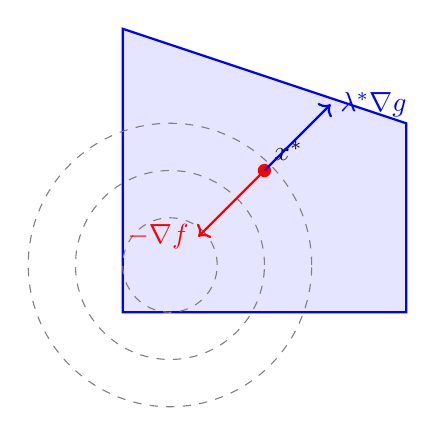
\begin{tikzpicture}[scale=1.2]
    % 可行域
    \fill[blue!10] (0, 0) -- (3, 0) -- (3, 2) -- (0, 3) -- cycle;
    \draw[blue, thick] (0, 0) -- (3, 0) -- (3, 2) -- (0, 3) -- cycle;
    
    % 等高线
    \draw[gray, dashed] (0.5, 0.5) circle (0.5);
    \draw[gray, dashed] (0.5, 0.5) circle (1);
    \draw[gray, dashed] (0.5, 0.5) circle (1.5);
    
    % 最优点
    \fill[red] (1.5, 1.5) circle (2pt);
    \node[above right] at (1.5, 1.5) {$x^*$};
    
    % 梯度
    \draw[->, thick, red] (1.5, 1.5) -- (0.8, 0.8);
    \node[left, red] at (0.8, 0.8) {$-\nabla f$};
    
    \draw[->, thick, blue] (1.5, 1.5) -- (2.2, 2.2);
    \node[right, blue] at (2.2, 2.2) {$\lambda^* \nabla g$};
\end{tikzpicture}
\end{center}

\textbf{互补松弛}：$\lambda_i^* g_i(x^*) = 0$

\begin{itemize}
    \item 如果约束不紧（$g_i(x^*) < 0$），则 $\lambda_i^* = 0$（约束``不起作用''）
    \item 如果 $\lambda_i^* > 0$，则约束必须紧（$g_i(x^*) = 0$）
\end{itemize}

\end{blackboard}

\begin{blackboard}[例子：带约束的二次规划]

\textbf{问题}：
\[
\min_x \frac{1}{2}x^2 \quad \text{s.t.} \quad x \geq 1
\]

\textbf{转换}：$g(x) = 1 - x \leq 0$

\textbf{Lagrangian}：$L(x, \lambda) = \frac{1}{2}x^2 + \lambda(1 - x)$

\textbf{KKT 条件}：
\begin{enumerate}
    \item 原始可行：$x \geq 1$
    \item 对偶可行：$\lambda \geq 0$
    \item 互补松弛：$\lambda(1 - x) = 0$
    \item 稳定性：$x - \lambda = 0$
\end{enumerate}

\textbf{求解}：由稳定性 $\lambda = x$。由互补松弛，要么 $\lambda = 0$（则 $x = 0$，违反原始可行），要么 $x = 1$。

故 $x^* = 1$，$\lambda^* = 1$。

\end{blackboard}

%========================================
\section{对偶的经济学解释}
%========================================

\begin{blackboard}[影子价格：约束的边际价值]

考虑带扰动的优化问题：
\[
\begin{aligned}
p^*(\epsilon) = \min_x \quad & f(x) \\
\text{s.t.} \quad & g_i(x) \leq \epsilon_i, \quad i = 1, \ldots, m
\end{aligned}
\]

当 $\epsilon = 0$ 时，就是原问题，最优值为 $p^*(0)$

\textbf{问题}：如果把第 $i$ 个约束放松一点（$\epsilon_i > 0$），最优值会改善多少？

\end{blackboard}

\begin{blackboard}[影子价格定理]

\begin{theorem}[影子价格]
在最优解处，对偶变量 $\lambda_i^*$ 满足：
\[
\lambda_i^* = -\frac{\partial p^*}{\partial \epsilon_i} \bigg|_{\epsilon = 0}
\]
\end{theorem}

\textbf{直觉}：$\lambda_i^*$ 告诉你``放松约束 $i$ 一个单位，目标函数能改善多少''

\textbf{近似公式}：当 $\epsilon$ 很小时
\[
p^*(\epsilon) \approx p^*(0) - \sum_{i=1}^m \lambda_i^* \epsilon_i
\]

\end{blackboard}

\begin{blackboard}[具体例子：生产问题]

\textbf{问题}：最小化成本，受资源约束
\[
\begin{aligned}
\min_x \quad & 2x_1 + 3x_2 \quad \text{（成本）} \\
\text{s.t.} \quad & x_1 + x_2 \geq 10 \quad \text{（产量需求）} \\
& x_1 \leq 8 \quad \text{（机器A产能）} \\
& x_2 \leq 6 \quad \text{（机器B产能）} \\
& x_1, x_2 \geq 0
\end{aligned}
\]

\textbf{转换为标准形式}（$g_i(x) \leq 0$）：
\begin{align*}
g_1(x) &= -x_1 - x_2 + 10 \leq 0 \quad \text{（产量约束）} \\
g_2(x) &= x_1 - 8 \leq 0 \quad \text{（机器A）} \\
g_3(x) &= x_2 - 6 \leq 0 \quad \text{（机器B）}
\end{align*}

\textbf{最优解}：$x_1^* = 4$，$x_2^* = 6$，成本 $= 2(4) + 3(6) = 26$

\end{blackboard}

\begin{blackboard}[影子价格的计算与解释]

\textbf{KKT 条件给出}：$\lambda_1^* = 2$，$\lambda_2^* = 0$，$\lambda_3^* = 1$

\textbf{解释}：

\textbf{约束1}（产量需求 $\geq 10$）：$\lambda_1^* = 2$
\begin{itemize}
    \item 如果只需要生产 9 件（放松 1 单位）
    \item 新问题：$g_1(x) = -x_1 - x_2 + 10 \leq 1$
    \item 成本减少约 $\lambda_1^* \times 1 = 2$ 元
\end{itemize}

\textbf{约束2}（机器A产能 $\leq 8$）：$\lambda_2^* = 0$
\begin{itemize}
    \item 当前 $x_1^* = 4 < 8$，产能没用完
    \item 增加机器A产能没有价值！
\end{itemize}

\textbf{约束3}（机器B产能 $\leq 6$）：$\lambda_3^* = 1$
\begin{itemize}
    \item 当前 $x_2^* = 6$，产能用尽
    \item 如果机器B产能增加到 7（放松 1 单位）
    \item 新问题：$g_3(x) = x_2 - 6 \leq 1$
    \item 成本减少约 $\lambda_3^* \times 1 = 1$ 元
\end{itemize}

\end{blackboard}

\begin{blackboard}[验证：放松约束后重新求解]

\textbf{原问题}：机器B产能 $\leq 6$
\begin{itemize}
    \item 最优解：$x_1^* = 4$，$x_2^* = 6$
    \item 成本：$26$
\end{itemize}

\textbf{放松后}：机器B产能 $\leq 7$
\begin{itemize}
    \item 新最优解：$x_1^* = 3$，$x_2^* = 7$
    \item 新成本：$2(3) + 3(7) = 27$？
\end{itemize}

等等，成本增加了？让我们重新思考...

\textbf{注意}：我们是在\textbf{最小化}成本，放松产能约束不一定降低成本！

\textbf{正确理解}：
\begin{itemize}
    \item $\lambda_3^* = 1$ 意味着约束``值 1 元''
    \item 如果\textbf{收紧}约束（机器B只能生产5件），成本会\textbf{增加}约 1 元
    \item 验证：$x_1 = 5, x_2 = 5$，成本 $= 2(5) + 3(5) = 25$... 
\end{itemize}

\textbf{重新审视}：影子价格的符号取决于问题的设定方式！

\end{blackboard}

\begin{blackboard}[影子价格的正确理解]

\textbf{关键公式}：
\[
p^*(\epsilon) \approx p^*(0) - \lambda^{*T} \epsilon
\]

\textbf{对于最小化问题}：
\begin{itemize}
    \item $\epsilon_i > 0$（放松约束）$\Rightarrow$ 可行域变大 $\Rightarrow$ $p^*$ 可能变小
    \item $\lambda_i^* \geq 0$，所以 $-\lambda_i^* \epsilon_i \leq 0$
\end{itemize}

\textbf{经济学直觉}：
\begin{itemize}
    \item $\lambda_i^*$ = 约束 $i$ 的``影子价格''
    \item = 你愿意为``放松约束一个单位''支付的最高价格
    \item = 约束的边际成本
\end{itemize}

\textbf{实际应用}：
\begin{itemize}
    \item 生产计划：应该购买哪种资源？（看哪个 $\lambda_i^*$ 最大）
    \item 电力市场：边际发电成本
    \item 物流优化：运力瓶颈在哪？
\end{itemize}

\end{blackboard}

\begin{blackboard}[互补松弛的经济学意义]

\textbf{互补松弛}：$\lambda_i^* g_i(x^*) = 0$

\textbf{翻译成人话}：

\begin{center}
\begin{tabular}{c|c|c}
情况 & 数学 & 经济学 \\
\hline
资源有剩余 & $g_i(x^*) < 0$ & 供过于求 \\
$\Rightarrow$ 价格为零 & $\lambda_i^* = 0$ & 免费资源无价值 \\
\hline
资源有价值 & $\lambda_i^* > 0$ & 稀缺资源 \\
$\Rightarrow$ 资源用尽 & $g_i(x^*) = 0$ & 供不应求
\end{tabular}
\end{center}

\textbf{直觉}：只有\textbf{稀缺}的资源才有价格！

\end{blackboard}

\begin{insight}[SVM 中的支持向量]

\textbf{SVM 对偶问题}的变量 $\alpha_i$ 就是 Lagrange 乘子

\textbf{互补松弛}：$\alpha_i (1 - y_i(w^T x_i + b)) = 0$

\begin{itemize}
    \item $\alpha_i = 0$：点 $x_i$ 不在边界上（不是支持向量）
    \item $\alpha_i > 0$：点 $x_i$ 恰好在边界上（是支持向量）
\end{itemize}

\textbf{结论}：只有\textbf{支持向量}对决策边界有贡献！

\begin{center}
\begin{tikzpicture}[scale=0.8]
    % 决策边界
    \draw[thick, blue] (-0.5, -2) -- (3.5, 2);
    \draw[dashed, blue] (-0.5, -1) -- (3.5, 3);
    \draw[dashed, blue] (-0.5, -3) -- (3.5, 1);
    
    % 正例
    \fill[red] (0, 1) circle (3pt);
    \fill[red] (0.5, 2) circle (3pt);
    \fill[red] (1, 1.5) circle (3pt);
    \draw[red, thick] (1, 1.5) circle (6pt); % 支持向量
    
    % 负例
    \fill[green!50!black] (2, -1) circle (3pt);
    \fill[green!50!black] (2.5, 0) circle (3pt);
    \fill[green!50!black] (3, -0.5) circle (3pt);
    \draw[green!50!black, thick] (2.5, 0) circle (6pt); % 支持向量
    
    \node[right] at (3.8, 2) {$\alpha_i > 0$};
    \node[right] at (3.8, 1.2) {支持向量};
\end{tikzpicture}
\end{center}

\end{insight}

%========================================
\section{机器学习视角：凸优化的现代应用}
%========================================

\begin{blackboard}[机器学习 = 优化]

几乎所有机器学习都可以写成：
\[
\min_\theta \underbrace{\frac{1}{n} \sum_{i=1}^n \ell(f_\theta(x_i), y_i)}_{\text{经验风险}} + \underbrace{\lambda R(\theta)}_{\text{正则化}}
\]

\begin{center}
\begin{tabular}{c|c|c}
模型 & 损失函数 $\ell$ & 正则化 $R$ \\
\hline
线性回归 & $(y - w^Tx)^2$ & $\|w\|_2^2$（岭回归） \\
Logistic 回归 & $\log(1 + e^{-y \cdot w^Tx})$ & $\|w\|_2^2$ 或 $\|w\|_1$ \\
SVM & $\max(0, 1 - y \cdot w^Tx)$ & $\|w\|_2^2$ \\
神经网络 & 交叉熵 & $\|W\|_F^2$（weight decay）
\end{tabular}
\end{center}

\textbf{关键问题}：哪些是凸的？哪些不是？

\end{blackboard}

\begin{blackboard}[凸 vs 非凸机器学习]

\begin{center}
\begin{tabular}{c|c|c}
& \textbf{凸} & \textbf{非凸} \\
\hline
\textbf{模型} & 线性回归、Logistic、SVM & 神经网络、矩阵分解 \\
& Lasso、岭回归 & 深度学习 \\
\hline
\textbf{优点} & 全局最优保证 & 表达能力强 \\
& 理论完善 & 能学复杂模式 \\
\hline
\textbf{缺点} & 表达能力有限 & 可能陷入局部最优 \\
& 只能学线性边界 & 理论不完善 \\
\hline
\textbf{优化方法} & 内点法、坐标下降 & SGD、Adam \\
& 精确解或收敛保证 & 启发式，实践有效
\end{tabular}
\end{center}

\end{blackboard}

\begin{blackboard}[为什么深度学习``不需要''凸优化？]

\textbf{传统观点}：非凸 = 噩梦（局部最优、鞍点）

\textbf{现代发现}：深度网络的损失景观有特殊结构

\begin{enumerate}
    \item \textbf{过参数化}：参数远多于数据，存在很多全局最优
    \item \textbf{鞍点主导}：高维空间中，局部最优很少，大多是鞍点
    \item \textbf{好的局部最优}：即使是局部最优，泛化性能也很好
    \item \textbf{隐式正则化}：SGD 本身倾向于找``平坦''的最优解
\end{enumerate}

\begin{center}
\begin{tikzpicture}[scale=0.6]
    % 低维：很多局部最优
    \begin{scope}
        \draw[->] (0, 0) -- (5, 0);
        \draw[->] (0, 0) -- (0, 3);
        \draw[thick, blue, domain=0.2:4.8, samples=100] plot (\x, {1 + 0.5*sin(3*\x r) + 0.3*sin(7*\x r)});
        \node[below] at (2.5, -0.3) {低维：很多局部最优};
    \end{scope}
    
    % 高维：鞍点主导
    \begin{scope}[xshift=7cm]
        \draw[->] (0, 0) -- (5, 0);
        \draw[->] (0, 0) -- (0, 3);
        \draw[thick, blue, domain=0.2:4.8, samples=100] plot (\x, {2 - 0.3*(\x-2.5)*(\x-2.5) + 0.5});
        \fill[red] (2.5, 2.5) circle (2pt);
        \node[above, red] at (2.5, 2.5) {鞍点};
        \node[below] at (2.5, -0.3) {高维：鞍点主导};
    \end{scope}
\end{tikzpicture}
\end{center}

\textbf{但是}：凸优化的思想仍然重要！

\end{blackboard}

\begin{blackboard}[凸优化思想在深度学习中的应用]

\textbf{1. 分层凸松弛}

神经网络训练非凸，但每一层固定其他层后是凸的：
\begin{itemize}
    \item 固定 $W_2$，优化 $W_1$：凸问题
    \item 交替优化：坐标下降的思想
\end{itemize}

\textbf{2. 正则化 = 凸约束}

$L_2$ 正则化：$\min \text{Loss} + \lambda \|w\|_2^2$

等价于约束优化：$\min \text{Loss}$ s.t. $\|w\|_2 \leq R$

对偶变量 $\lambda$ = 约束的影子价格！

\textbf{3. 对偶在 Kernel 方法中的核心作用}

SVM 对偶：
\[
\max_\alpha \sum_i \alpha_i - \frac{1}{2} \sum_{i,j} \alpha_i \alpha_j y_i y_j K(x_i, x_j)
\]

核技巧（Kernel Trick）完全依赖对偶形式！

\textbf{4. KKT 条件 $\to$ 最优性检验}

即使用 SGD 训练，也可以用 KKT 残差判断是否收敛

\end{blackboard}

\begin{blackboard}[现代机器学习中的凸子问题]

\textbf{很多非凸问题包含凸子问题}：

\begin{center}
\begin{tabular}{c|c}
\textbf{问题} & \textbf{凸子问题} \\
\hline
神经网络训练 & 最后一层是凸的（固定特征） \\
EM 算法 & M-step 通常是凸的 \\
矩阵分解 & 固定一个因子，另一个是凸的 \\
变分推断 & ELBO 优化常是凸的 \\
强化学习 & Policy evaluation 是线性方程 \\
对抗训练 & 内层 max 可能是凸的
\end{tabular}
\end{center}

\textbf{启示}：理解凸优化 = 理解复杂系统的``积木块''

\end{blackboard}

\begin{blackboard}[Logistic 回归的凸性证明 $\bigstar$]

\textbf{损失函数}：
\[
L(w) = \sum_{i=1}^n \log(1 + e^{-y_i w^T x_i})
\]

\textbf{要证}：$L(w)$ 是凸函数

\textbf{证明}：设 $\ell(z) = \log(1 + e^{-z})$，则 $L(w) = \sum_i \ell(y_i w^T x_i)$

\textbf{Step 1}：证明 $\ell(z)$ 是凸的
\[
\ell'(z) = \frac{-e^{-z}}{1 + e^{-z}} = \frac{-1}{1 + e^z} = -(1 - \sigma(z))
\]
\[
\ell''(z) = \sigma(z)(1 - \sigma(z)) \geq 0 \quad \checkmark
\]

\textbf{Step 2}：$\ell(y_i w^T x_i)$ 是 $w$ 的凸函数

因为 $y_i w^T x_i$ 是 $w$ 的仿射函数，凸函数复合仿射仍是凸

\textbf{Step 3}：凸函数的和是凸函数 \hfill $\square$

\textbf{加上正则化}：$L(w) + \lambda \|w\|_2^2$ 是\textbf{强凸}的（$\lambda > 0$）

\end{blackboard}

%========================================
\section{MDP 与线性规划 $\bigstar$}
%========================================

\begin{blackboard}[从实际问题出发]

\textbf{问题1：库存管理}

你经营一家书店，每天要决定进多少货：
\begin{itemize}
    \item 进多了：库存成本高，书可能卖不掉
    \item 进少了：缺货损失销售机会
    \item 需求是随机的（今天可能卖 10 本，也可能卖 50 本）
\end{itemize}

\textbf{问题2：机器维护}

你管理一台机器，每天要决定是否维护：
\begin{itemize}
    \item 机器有``好''``中''``差''三种状态
    \item 不维护：省钱，但机器可能变差
    \item 维护：花钱，但机器变好
    \item 机器太差会坏掉，损失更大
\end{itemize}

\textbf{问题3：走迷宫}

机器人在网格中找出口：
\begin{itemize}
    \item 每一步可以上下左右移动
    \item 有些格子是障碍物
    \item 目标：用最少步数到达出口
\end{itemize}

\textbf{共同特点}：状态 $\to$ 决策 $\to$ 随机转移 $\to$ 新状态 $\to$ ...

\end{blackboard}

\begin{blackboard}[什么是马尔可夫性？]

\textbf{马尔可夫性}（Markov Property）：未来只依赖于现在，与过去无关

\[
P(s_{t+1} | s_t, s_{t-1}, \ldots, s_0) = P(s_{t+1} | s_t)
\]

\textbf{例子：天气}

\begin{center}
\begin{tikzpicture}[scale=0.9, 
    state/.style={circle, draw, minimum size=1.2cm},
    every edge/.style={draw, ->, >=stealth, thick}]
    
    \node[state, fill=yellow!30] (sunny) at (0, 0) {晴};
    \node[state, fill=gray!30] (rainy) at (4, 0) {雨};
    
    \draw (sunny) edge[loop above] node[above] {0.8} (sunny);
    \draw (sunny) edge[bend left] node[above] {0.2} (rainy);
    \draw (rainy) edge[bend left] node[below] {0.4} (sunny);
    \draw (rainy) edge[loop above] node[above] {0.6} (rainy);
\end{tikzpicture}
\end{center}

明天是否下雨，只取决于今天的天气，不取决于昨天、前天...

\textbf{马尔可夫链}：状态按概率转移，没有决策

\textbf{马尔可夫决策过程 (MDP)}：加入决策！你可以选择动作影响转移

\end{blackboard}

\begin{blackboard}[MDP 的正式定义]

\textbf{MDP} = $(S, A, P, R, \gamma)$

\begin{itemize}
    \item $S$：状态空间（有限集合 $\{1, 2, \ldots, n\}$）
    \item $A$：动作空间（有限集合）
    \item $P(s' | s, a)$：转移概率（在状态 $s$ 执行动作 $a$ 后到达 $s'$ 的概率）
    \item $R(s, a)$：即时奖励（在状态 $s$ 执行动作 $a$ 获得的奖励）
    \item $\gamma \in [0, 1)$：折扣因子（未来奖励的衰减）
\end{itemize}

\textbf{策略}：$\pi: S \to A$，告诉你在每个状态该做什么

\textbf{目标}：找最优策略 $\pi^*$，最大化累积折扣奖励
\[
\mathbb{E}\left[ \sum_{t=0}^\infty \gamma^t R(s_t, a_t) \right]
\]

\textbf{为什么要折扣？}
\begin{itemize}
    \item 今天的 1 元比明天的 1 元更值钱
    \item 数学上保证级数收敛
    \item $\gamma$ 接近 1：更有远见；$\gamma$ 接近 0：更短视
\end{itemize}

\end{blackboard}

\subsection{具体例子：机器维护问题}

\begin{blackboard}[机器维护 MDP]

\textbf{状态}：$S = \{\text{好}, \text{中}, \text{差}\}$

\textbf{动作}：$A = \{\text{不维护}, \text{维护}\}$

\textbf{转移概率}（不维护时机器会慢慢变差）：

\begin{center}
\begin{tabular}{c|ccc}
$P(\cdot | s, \text{不维护})$ & 好 & 中 & 差 \\
\hline
好 & 0.7 & 0.3 & 0 \\
中 & 0 & 0.6 & 0.4 \\
差 & 0 & 0 & 1
\end{tabular}
\quad
\begin{tabular}{c|ccc}
$P(\cdot | s, \text{维护})$ & 好 & 中 & 差 \\
\hline
好 & 1 & 0 & 0 \\
中 & 0.5 & 0.5 & 0 \\
差 & 0.2 & 0.6 & 0.2
\end{tabular}
\end{center}

\textbf{奖励}（好机器生产多，维护要花钱）：

\begin{center}
\begin{tabular}{c|cc}
$R(s, a)$ & 不维护 & 维护 \\
\hline
好 & 10 & 7 \\
中 & 5 & 2 \\
差 & -1 & -4
\end{tabular}
\end{center}

\textbf{问题}：应该什么时候维护？

\end{blackboard}

\begin{blackboard}[机器维护：两种策略对比]

\textbf{策略1}：从不维护
\begin{itemize}
    \item 短期省钱
    \item 长期机器变差，损失大
\end{itemize}

\textbf{策略2}：状态``中''或``差''时维护
\begin{itemize}
    \item 维护有成本
    \item 但机器保持好状态，长期收益高
\end{itemize}

\textbf{哪个更好？} 需要计算！

设 $\gamma = 0.9$，我们来求最优策略...

\end{blackboard}

\subsection{Bellman 方程}

\begin{blackboard}[值函数：衡量状态的好坏]

\begin{definition}[状态值函数]
策略 $\pi$ 下，从状态 $s$ 出发的期望累积奖励：
\[
V^\pi(s) = \mathbb{E}_\pi \left[ \sum_{t=0}^\infty \gamma^t R(s_t, \pi(s_t)) \mid s_0 = s \right]
\]
\end{definition}

\textbf{直觉}：$V^\pi(s)$ 告诉你``从状态 $s$ 出发，按策略 $\pi$ 走，期望能拿多少奖励''

\textbf{最优值函数}：
\[
V^*(s) = \max_\pi V^\pi(s)
\]

这是所有策略中能达到的最大值

\end{blackboard}

\begin{blackboard}[Bellman 方程：递归结构]

\begin{theorem}[Bellman 期望方程]
\[
V^\pi(s) = R(s, \pi(s)) + \gamma \sum_{s'} P(s' | s, \pi(s)) V^\pi(s')
\]
\end{theorem}

\textbf{翻译}：从 $s$ 出发的总价值 = 立即奖励 + 折扣 $\times$ 下一状态的期望价值

\begin{theorem}[Bellman 最优方程]
\[
V^*(s) = \max_a \left[ R(s, a) + \gamma \sum_{s'} P(s' | s, a) V^*(s') \right]
\]
\end{theorem}

\textbf{翻译}：最优价值 = 选择最好的动作，获得立即奖励 + 折扣 $\times$ 下一状态的最优价值

\end{blackboard}

\begin{blackboard}[机器维护：计算值函数]

设 $\gamma = 0.9$，Bellman 最优方程：

\textbf{状态``好''}：
\[
V^*(\text{好}) = \max \begin{cases}
10 + 0.9 (0.7 V^*(\text{好}) + 0.3 V^*(\text{中})) & \text{不维护} \\
7 + 0.9 \cdot V^*(\text{好}) & \text{维护}
\end{cases}
\]

\textbf{状态``中''}：
\[
V^*(\text{中}) = \max \begin{cases}
5 + 0.9 (0.6 V^*(\text{中}) + 0.4 V^*(\text{差})) & \text{不维护} \\
2 + 0.9 (0.5 V^*(\text{好}) + 0.5 V^*(\text{中})) & \text{维护}
\end{cases}
\]

\textbf{状态``差''}：
\[
V^*(\text{差}) = \max \begin{cases}
-1 + 0.9 \cdot V^*(\text{差}) & \text{不维护} \\
-4 + 0.9 (0.2 V^*(\text{好}) + 0.6 V^*(\text{中}) + 0.2 V^*(\text{差})) & \text{维护}
\end{cases}
\]

这是一个非线性方程组（因为有 max）... 如何求解？

\end{blackboard}

\subsection{MDP 的线性规划形式}

\begin{blackboard}[关键观察：把 max 变成不等式]

Bellman 最优方程：
\[
V^*(s) = \max_a \left[ R(s, a) + \gamma \sum_{s'} P(s'|s,a) V^*(s') \right]
\]

\textbf{等价于}：$V^*(s)$ 是满足以下条件的\textbf{最小}的 $V$

对所有状态 $s$ 和动作 $a$：
\[
V(s) \geq R(s, a) + \gamma \sum_{s'} P(s'|s,a) V(s')
\]

\textbf{为什么？}
\begin{itemize}
    \item $V^*$ 显然满足这些不等式（因为 max $\geq$ 任何一项）
    \item 如果 $V$ 满足所有不等式且 $V < V^*$，则存在某个 $s$ 使得
    
    $V(s) < V^*(s) = R(s, a^*) + \gamma \sum_{s'} P(s'|s,a^*) V^*(s')$
    
    但 $V(s) \geq R(s, a^*) + \gamma \sum_{s'} P(s'|s,a^*) V(s') \geq R(s, a^*) + \gamma \sum_{s'} P(s'|s,a^*) V^*(s')$
    
    矛盾！
\end{itemize}

\end{blackboard}

\begin{blackboard}[MDP 的 LP 形式]

\begin{theorem}[MDP 的线性规划]
最优值函数 $V^*$ 是以下 LP 的解：
\[
\begin{aligned}
\min_V \quad & \sum_s \mu(s) V(s) \\
\text{s.t.} \quad & V(s) \geq R(s,a) + \gamma \sum_{s'} P(s'|s,a) V(s'), \quad \forall s \in S, \forall a \in A
\end{aligned}
\]
其中 $\mu(s) > 0$ 是任意正的权重。
\end{theorem}

\textbf{这是一个标准的 LP！}
\begin{itemize}
    \item 变量：$V(s)$，共 $|S|$ 个
    \item 约束：每对 $(s, a)$ 一个，共 $|S| \times |A|$ 个
    \item 目标：线性
    \item 约束：线性
\end{itemize}

\textbf{可以用单纯形法或内点法求解！}

\end{blackboard}

\begin{blackboard}[机器维护问题的 LP]

状态：好(G)、中(M)、差(B)，动作：不维护(N)、维护(R)

\textbf{变量}：$V_G, V_M, V_B$

\textbf{LP}（取 $\mu = (1/3, 1/3, 1/3)$）：
\[
\min \frac{1}{3}(V_G + V_M + V_B)
\]

\textbf{约束}（6 个，每个 $(s,a)$ 一个）：
\begin{align*}
V_G &\geq 10 + 0.9(0.7 V_G + 0.3 V_M) & \text{(好, 不维护)} \\
V_G &\geq 7 + 0.9 V_G & \text{(好, 维护)} \\
V_M &\geq 5 + 0.9(0.6 V_M + 0.4 V_B) & \text{(中, 不维护)} \\
V_M &\geq 2 + 0.9(0.5 V_G + 0.5 V_M) & \text{(中, 维护)} \\
V_B &\geq -1 + 0.9 V_B & \text{(差, 不维护)} \\
V_B &\geq -4 + 0.9(0.2 V_G + 0.6 V_M + 0.2 V_B) & \text{(差, 维护)}
\end{align*}

\end{blackboard}

\begin{blackboard}[用 CVXPY 求解]

\begin{lstlisting}[language=Python]
import cvxpy as cp
import numpy as np

# 变量
V = cp.Variable(3)  # V[0]=V_G, V[1]=V_M, V[2]=V_B
gamma = 0.9

# 目标
obj = cp.Minimize(cp.sum(V) / 3)

# 约束
constraints = [
    # 状态 好
    V[0] >= 10 + gamma * (0.7*V[0] + 0.3*V[1]),  # 不维护
    V[0] >= 7 + gamma * V[0],                     # 维护
    # 状态 中
    V[1] >= 5 + gamma * (0.6*V[1] + 0.4*V[2]),   # 不维护
    V[1] >= 2 + gamma * (0.5*V[0] + 0.5*V[1]),   # 维护
    # 状态 差
    V[2] >= -1 + gamma * V[2],                    # 不维护
    V[2] >= -4 + gamma * (0.2*V[0] + 0.6*V[1] + 0.2*V[2])  # 维护
]

prob = cp.Problem(obj, constraints)
prob.solve()
print(f"V* = {V.value}")  # [73.8, 64.5, 47.2] 大约
\end{lstlisting}

\end{blackboard}

\begin{blackboard}[从值函数恢复最优策略]

\textbf{求解 LP 得到}：$V^*_G \approx 73.8$，$V^*_M \approx 64.5$，$V^*_B \approx 47.2$

\textbf{最优策略}：选择使 Bellman 方程取等的动作

\textbf{状态``好''}：
\begin{itemize}
    \item 不维护：$10 + 0.9(0.7 \times 73.8 + 0.3 \times 64.5) \approx 73.8$ \checkmark
    \item 维护：$7 + 0.9 \times 73.8 \approx 73.4$
\end{itemize}
$\Rightarrow$ \textbf{不维护}

\textbf{状态``中''}：
\begin{itemize}
    \item 不维护：$5 + 0.9(0.6 \times 64.5 + 0.4 \times 47.2) \approx 56.8$
    \item 维护：$2 + 0.9(0.5 \times 73.8 + 0.5 \times 64.5) \approx 64.5$ \checkmark
\end{itemize}
$\Rightarrow$ \textbf{维护}

\textbf{状态``差''}：
\begin{itemize}
    \item 不维护：$-1 + 0.9 \times 47.2 \approx 41.5$
    \item 维护：$-4 + 0.9(0.2 \times 73.8 + 0.6 \times 64.5 + 0.2 \times 47.2) \approx 47.2$ \checkmark
\end{itemize}
$\Rightarrow$ \textbf{维护}

\textbf{最优策略}：好 $\to$ 不维护，中 $\to$ 维护，差 $\to$ 维护

\end{blackboard}

\subsection{LP 对偶与占用度量}

\begin{blackboard}[MDP 的对偶 LP]

\textbf{原问题}有对偶！引入对偶变量 $\rho(s, a) \geq 0$

\begin{theorem}[MDP 的对偶 LP]
\[
\begin{aligned}
\max_\rho \quad & \sum_{s,a} \rho(s,a) R(s,a) \\
\text{s.t.} \quad & \sum_a \rho(s,a) = \mu(s) + \gamma \sum_{s',a'} \rho(s',a') P(s|s',a'), \quad \forall s \\
& \rho(s,a) \geq 0
\end{aligned}
\]
\end{theorem}

\textbf{$\rho(s,a)$ 的含义}：\textbf{占用度量}（Occupancy Measure）

$\rho(s,a)$ = 在最优策略下，处于状态 $s$ 并执行动作 $a$ 的（折扣）频率

\end{blackboard}

\begin{blackboard}[对偶约束的直觉：流量守恒]

约束：$\sum_a \rho(s,a) = \mu(s) + \gamma \sum_{s',a'} \rho(s',a') P(s|s',a')$

\textbf{翻译}：
\[
\underbrace{\sum_a \rho(s,a)}_{\text{从 } s \text{ 流出}} = \underbrace{\mu(s)}_{\text{初始流入}} + \underbrace{\gamma \sum_{s',a'} \rho(s',a') P(s|s',a')}_{\text{从其他状态转移来}}
\]

\begin{center}
\begin{tikzpicture}[scale=0.9]
    \node[draw, circle, fill=blue!20, minimum size=1.5cm] (s) at (0, 0) {$s$};
    
    % 流入
    \draw[->, thick, red] (-3, 1) -- (s) node[midway, above] {$\mu(s)$};
    \draw[->, thick, orange] (-3, -0.5) -- (s) node[midway, below] {从 $s'$ 来};
    
    % 流出
    \draw[->, thick, blue] (s) -- (3, 0.5) node[midway, above] {$\rho(s, a_1)$};
    \draw[->, thick, blue] (s) -- (3, -0.5) node[midway, below] {$\rho(s, a_2)$};
    
    \node at (0, -2) {流入 = 流出};
\end{tikzpicture}
\end{center}

\textbf{这就是网络流的守恒定律！}

\end{blackboard}

\begin{blackboard}[原问题 vs 对偶问题]

\begin{center}
\begin{tabular}{c|c|c}
& \textbf{原问题} & \textbf{对偶问题} \\
\hline
\textbf{变量} & $V(s)$：值函数 & $\rho(s,a)$：占用度量 \\
\textbf{数量} & $|S|$ 个 & $|S| \times |A|$ 个 \\
\textbf{约束} & Bellman 不等式 & 流量守恒 \\
\textbf{目标} & 最小化总值 & 最大化总奖励 \\
\textbf{视角} & ``状态有多好？'' & ``应该怎么做？''
\end{tabular}
\end{center}

\textbf{强对偶}：两个 LP 的最优值相等！（凸优化的对偶理论）

\textbf{从对偶解恢复策略}：
\[
\pi^*(a|s) = \frac{\rho^*(s,a)}{\sum_{a'} \rho^*(s,a')}
\]

\end{blackboard}

\begin{blackboard}[互补松弛在 MDP 中的意义]

\textbf{KKT 互补松弛}：$\rho^*(s,a) \cdot \left[ V^*(s) - R(s,a) - \gamma \sum_{s'} P(s'|s,a) V^*(s') \right] = 0$

\textbf{翻译}：
\begin{itemize}
    \item 如果 $\rho^*(s,a) > 0$（动作 $a$ 在状态 $s$ 被执行）
    
    $\Rightarrow$ Bellman 不等式取等（$a$ 是最优动作）
    
    \item 如果动作 $a$ 不是最优的（Bellman 不等式严格）
    
    $\Rightarrow$ $\rho^*(s,a) = 0$（这个动作不会被执行）
\end{itemize}

\textbf{经济学解释}：
\begin{itemize}
    \item $V^*(s)$ = 状态 $s$ 的``影子价格''
    \item 只有``物有所值''的动作才会被使用
    \item 次优动作的``使用量''为零
\end{itemize}

\end{blackboard}

\begin{insight}[MDP-LP 总结]

\textbf{核心结论}：
\begin{itemize}
    \item MDP 的最优策略可以通过 LP 精确求解
    \item 原问题变量是值函数，对偶变量是占用度量
    \item LP 对偶揭示了``评估''与``决策''的深层联系
\end{itemize}

\textbf{为什么这很重要？}
\begin{itemize}
    \item 把决策问题转化为我们熟悉的凸优化
    \item KKT 条件给出最优性的刻画
    \item 影子价格、互补松弛都有自然解释
\end{itemize}

\textbf{局限性}：
\begin{itemize}
    \item 需要知道完整的 MDP 模型（$P$, $R$）
    \item 状态空间大时（如围棋 $10^{170}$ 状态），LP 不可行
    \item 实际中常用近似方法（值迭代、策略迭代、函数逼近）
\end{itemize}

\textbf{但 LP 视角提供了理论基础！}

\end{insight}

%========================================
\section{GPU 改变现代优化}
%========================================

\begin{blackboard}[经典优化 vs 现代优化]

\textbf{经典优化}（1960s-2000s）：

\begin{itemize}
    \item 内点法、单纯形法
    \item 每步计算量大，但步数少
    \item 适合中等规模问题（$n < 10^5$）
    \item 需要精确的二阶信息（Hessian）
\end{itemize}

\textbf{现代优化}（2010s-）：

\begin{itemize}
    \item 随机梯度下降（SGD）及其变体
    \item 每步计算量小，但步数多
    \item 适合超大规模问题（$n > 10^9$）
    \item 只需要一阶信息（梯度）
\end{itemize}

\textbf{为什么变了？}

\end{blackboard}

\begin{gpubox}[GPU 的出现改变了游戏规则]

\textbf{内点法的瓶颈}：

每步需要解线性系统 $H \Delta x = -g$，其中 $H$ 是 Hessian

\begin{itemize}
    \item 形成 $H$：$O(n^2)$ 存储
    \item 求解线性系统：$O(n^3)$ 或稀疏情况 $O(n^{1.5})$
    \item \textbf{很难并行化}
\end{itemize}

\textbf{梯度下降的优势}：

每步只需计算 $x \leftarrow x - \alpha \nabla f(x)$

\begin{itemize}
    \item 只需 $O(n)$ 存储
    \item 计算梯度：可以高度并行化
    \item \textbf{完美匹配 GPU 架构}
\end{itemize}

\end{gpubox}

\begin{blackboard}[数值对比]

\textbf{问题}：$n = 10^6$ 变量的凸优化

\begin{center}
\begin{tabular}{c|c|c|c}
方法 & 每步复杂度 & 收敛步数 & 实际时间 \\
\hline
内点法 (CPU) & $O(n^3)$ & $\sim 50$ & 几天（内存不够） \\
梯度下降 (CPU) & $O(n)$ & $\sim 10^4$ & 几小时 \\
梯度下降 (GPU) & $O(n)$ 并行 & $\sim 10^4$ & \textbf{几分钟}
\end{tabular}
\end{center}

\textbf{深度学习的选择}：

神经网络参数量：$n \sim 10^9$（GPT-3 有 1750 亿参数）

内点法？绝对不可能。只能用 SGD + GPU。

\end{blackboard}

\begin{blackboard}[批量优化：GPU 的超能力]

\textbf{场景}：需要解 1000 个独立的小优化问题

\textbf{传统方法}（顺序）：
\begin{itemize}
    \item 每个问题 0.1 秒
    \item 总时间：$1000 \times 0.1 = 100$ 秒
\end{itemize}

\textbf{GPU 方法}（并行）：
\begin{itemize}
    \item 1000 个问题同时求解
    \item 总时间：$\approx 0.1$ 秒（几乎和 1 个问题一样）
\end{itemize}

\textbf{加速比}：$\sim 1000\times$

\textbf{应用}：
\begin{itemize}
    \item 强化学习：同时模拟 1000 个环境
    \item 超参数搜索：同时训练 1000 个模型
    \item 蒙特卡洛：同时采样 1000 条路径
\end{itemize}

\end{blackboard}

\begin{insight}[理论 vs 实践的张力]

\textbf{理论}说：

凸优化用内点法，$O(\sqrt{n})$ 步收敛，每步 $O(n^3)$

\textbf{实践}说：

管他收敛多少步，能在 GPU 上跑、能处理 $10^9$ 变量才是王道

\textbf{调和}：

\begin{itemize}
    \item 小问题（$n < 10^4$）：内点法仍是王者
    \item 大问题（$n > 10^6$）：一阶方法 + GPU
    \item 结构化问题：针对性算法（如 ADMM）
\end{itemize}

\textbf{本课程}：两种视角都要学，知道何时用哪种

\end{insight}

%========================================
\section{实验}
%========================================

\subsection{实验 2a：CVXPY 求解 SVM 对偶}

\begin{experiment}[观察 KKT 条件与支持向量]

\textbf{目标}：
\begin{itemize}
    \item 用 CVXPY 求解 SVM 对偶问题
    \item 观察互补松弛条件
    \item 识别支持向量
\end{itemize}

\textbf{SVM 原始问题}：
\[
\min_{w, b} \frac{1}{2}\|w\|^2 \quad \text{s.t.} \quad y_i(w^T x_i + b) \geq 1
\]

\textbf{SVM 对偶问题}：
\[
\max_{\alpha} \sum_i \alpha_i - \frac{1}{2} \sum_{i,j} \alpha_i \alpha_j y_i y_j x_i^T x_j \quad \text{s.t.} \quad \alpha_i \geq 0, \sum_i \alpha_i y_i = 0
\]

\end{experiment}

\begin{blackboard}[实验代码框架]

\begin{lstlisting}[language=Python]
import cvxpy as cp
import numpy as np

# 生成数据
np.random.seed(42)
n_samples = 50
X_pos = np.random.randn(n_samples//2, 2) + [2, 2]
X_neg = np.random.randn(n_samples//2, 2) + [-2, -2]
X = np.vstack([X_pos, X_neg])
y = np.array([1]*(n_samples//2) + [-1]*(n_samples//2))

# 对偶问题
n = len(y)
alpha = cp.Variable(n)
K = (X @ X.T) * np.outer(y, y)  # Gram 矩阵

objective = cp.Maximize(cp.sum(alpha) - 0.5 * cp.quad_form(alpha, K))
constraints = [alpha >= 0, alpha @ y == 0]
prob = cp.Problem(objective, constraints)
prob.solve()

# 找支持向量
alpha_val = alpha.value
support_vectors = np.where(alpha_val > 1e-5)[0]
print(f"支持向量数量: {len(support_vectors)}")
print(f"支持向量的 alpha: {alpha_val[support_vectors]}")
\end{lstlisting}

\end{blackboard}

\begin{blackboard}[观察互补松弛]

\textbf{KKT 互补松弛}：$\alpha_i (1 - y_i(w^T x_i + b)) = 0$

\begin{lstlisting}[language=Python]
# 从对偶解恢复原始变量
w = sum(alpha_val[i] * y[i] * X[i] for i in range(n))
# 从支持向量计算 b
sv_idx = support_vectors[0]
b = y[sv_idx] - w @ X[sv_idx]

# 验证互补松弛
for i in range(n):
    margin = y[i] * (w @ X[i] + b)
    slack = alpha_val[i] * (1 - margin)
    if alpha_val[i] > 1e-5:
        print(f"点 {i}: alpha={alpha_val[i]:.4f}, "
              f"margin={margin:.4f}, slack={slack:.6f}")
\end{lstlisting}

\textbf{预期结果}：
\begin{itemize}
    \item $\alpha_i > 0$ 的点：margin $\approx 1$（在边界上）
    \item $\alpha_i = 0$ 的点：margin $> 1$（远离边界）
\end{itemize}

\end{blackboard}

\subsection{实验 2b：GPU vs CPU 凸优化}

\begin{experiment}[规模与方法的权衡]

\textbf{目标}：比较不同规模下的最优策略

\begin{center}
\begin{tabular}{c|c|c}
规模 & 推荐方法 & 原因 \\
\hline
小 ($n \sim 100$) & CVXPY 内点法 & 精确、快速 \\
中 ($n \sim 10^4$) & 视情况 & 过渡区域 \\
大 ($n \sim 10^5+$) & GPU 梯度下降 & 内点法内存爆炸
\end{tabular}
\end{center}

\end{experiment}

\begin{blackboard}[实验代码：小规模 QP]

\begin{lstlisting}[language=Python]
import cvxpy as cp
import numpy as np
import time

# 小规模 QP: n = 100
n = 100
np.random.seed(42)
P = np.random.randn(n, n)
P = P.T @ P + 0.1 * np.eye(n)  # 确保正定
q = np.random.randn(n)

x = cp.Variable(n)
objective = cp.Minimize(0.5 * cp.quad_form(x, P) + q @ x)
constraints = [x >= 0]
prob = cp.Problem(objective, constraints)

start = time.time()
prob.solve()
print(f"CVXPY (n={n}): {time.time() - start:.4f} 秒")
print(f"最优值: {prob.value:.4f}")
\end{lstlisting}

\textbf{预期}：内点法在毫秒级完成

\end{blackboard}

\begin{blackboard}[实验代码：大规模 QP]

\begin{lstlisting}[language=Python]
import torch

# 大规模 QP: n = 50000
n = 50000
device = 'cuda' if torch.cuda.is_available() else 'cpu'

P = torch.randn(n, n, device=device)
P = P.T @ P + 0.1 * torch.eye(n, device=device)
q = torch.randn(n, device=device)

# 投影梯度下降
x = torch.zeros(n, device=device, requires_grad=True)
optimizer = torch.optim.Adam([x], lr=0.01)

start = time.time()
for i in range(1000):
    loss = 0.5 * x @ P @ x + q @ x
    optimizer.zero_grad()
    loss.backward()
    optimizer.step()
    with torch.no_grad():
        x.clamp_(min=0)  # 投影到 x >= 0
    
    if i % 200 == 0:
        print(f"Step {i}: loss = {loss.item():.4f}")

print(f"GPU 梯度下降 (n={n}): {time.time() - start:.2f} 秒")
\end{lstlisting}

\end{blackboard}

\begin{blackboard}[实验代码：批量优化]

\begin{lstlisting}[language=Python]
# 批量优化：同时解 1000 个独立的小 QP
batch_size = 1000
n = 100

# 生成 1000 个不同的问题
P_batch = torch.randn(batch_size, n, n, device=device)
P_batch = P_batch.transpose(-1, -2) @ P_batch 
P_batch = P_batch + 0.1 * torch.eye(n, device=device)
q_batch = torch.randn(batch_size, n, device=device)

x_batch = torch.zeros(batch_size, n, device=device, 
                      requires_grad=True)
optimizer = torch.optim.Adam([x_batch], lr=0.1)

start = time.time()
for i in range(500):
    # 批量计算所有问题的目标函数
    loss = 0.5 * torch.einsum('bi,bij,bj->b', 
                              x_batch, P_batch, x_batch)
    loss = loss + torch.einsum('bi,bi->b', q_batch, x_batch)
    loss = loss.sum()
    
    optimizer.zero_grad()
    loss.backward()
    optimizer.step()
    with torch.no_grad():
        x_batch.clamp_(min=0)

print(f"批量优化 1000 个问题: {time.time() - start:.2f} 秒")
\end{lstlisting}

\textbf{预期}：1000 个问题的时间 $\approx$ 1 个问题的时间

\end{blackboard}

%========================================
\section{本周总结}
%========================================

\begin{keypoint}[数学定理总结]

\textbf{凸性判定}（会证明 $\bigstar$）：
\begin{itemize}
    \item 一阶条件：$f(y) \geq f(x) + \nabla f(x)^T(y-x)$ $\Leftrightarrow$ $f$ 凸
    \item 二阶条件：$\nabla^2 f(x) \succeq 0$ 对所有 $x$ $\Leftrightarrow$ $f$ 凸
    \item 强凸：$\nabla^2 f(x) \succeq mI$，$m > 0$
\end{itemize}

\textbf{对偶理论}：
\begin{itemize}
    \item 弱对偶（总成立）：$d^* \leq p^*$
    \item 强对偶（Slater 条件）：$d^* = p^*$
    \item 对偶间隙：$p^* - d^* \geq 0$
\end{itemize}

\textbf{KKT 条件}（会推导 $\bigstar$）：
\begin{enumerate}
    \item 原始可行：$g_i(x^*) \leq 0$，$h_j(x^*) = 0$
    \item 对偶可行：$\lambda_i^* \geq 0$
    \item 互补松弛：$\lambda_i^* g_i(x^*) = 0$
    \item 稳定性：$\nabla_x L = 0$
\end{enumerate}

\end{keypoint}

\begin{keypoint}[现代视角]

\textbf{凸优化在机器学习中的地位}：
\begin{itemize}
    \item 经典 ML（SVM、Logistic、Lasso）：凸优化是核心
    \item 深度学习：非凸，但凸优化思想仍然重要
    \item 子问题：很多非凸问题包含凸子问题
\end{itemize}

\textbf{理论 vs 实践}：
\begin{itemize}
    \item 小规模（$n < 10^4$）：内点法，精确解
    \item 大规模（$n > 10^6$）：一阶方法 + GPU
    \item 批量问题：GPU 并行，1000 个 $\approx$ 1 个
\end{itemize}

\textbf{对偶的三重价值}：
\begin{enumerate}
    \item 提供下界（最优性证书）
    \item 影子价格（敏感性分析）
    \item 核技巧（SVM、Kernel 方法）
\end{enumerate}

\end{keypoint}

\begin{keypoint}[带走的核心技能]

\textbf{概念层面}：
\begin{itemize}
    \item 能判断一个优化问题是否是凸的
    \item 理解``凸 = 局部即全局''的意义
    \item 知道 KKT 条件的四个组成部分
\end{itemize}

\textbf{计算层面}：
\begin{itemize}
    \item 能写出简单问题的 Lagrangian
    \item 能用 KKT 条件手算小问题
    \item 能用 CVXPY 求解中等规模凸优化
\end{itemize}

\textbf{直觉层面}：
\begin{itemize}
    \item 互补松弛 = 稀缺资源才有价格
    \item 对偶变量 = 约束的边际价值
    \item 支持向量 = 对偶变量非零的点
\end{itemize}

\end{keypoint}

%========================================
\section{思考题}
%========================================

\begin{blackboard}[思考题]

\textbf{1.} 证明：如果 $f$ 和 $g$ 都是凸函数，则 $\max\{f(x), g(x)\}$ 也是凸函数。

\textbf{2.} 为什么凸优化的等式约束只能是仿射的？举一个反例说明非仿射等式约束会破坏凸性。

\textbf{3.} 考虑问题 $\min x^2$ s.t. $x \geq 2$。
\begin{itemize}
    \item[(a)] 写出 KKT 条件
    \item[(b)] 求解最优解和最优 Lagrange 乘子
    \item[(c)] 验证互补松弛条件
\end{itemize}

\textbf{4.} 在 SVM 中，如果所有训练样本都正确分类且远离边界，会发生什么？这时有多少支持向量？

\textbf{5.} 设计实验：对于 $n = 1000, 5000, 10000, 50000$ 的 QP 问题，分别用 CVXPY 内点法和 GPU 梯度下降求解，画出``问题规模 vs 求解时间''的曲线。在什么规模下 GPU 开始占优势？

\end{blackboard}

\end{document}